\section{Experiments and Results}
The three compression schemes were tested on the Wikipedia corpus (enwik8, enwik9), IMDB principal data and a protein FASTA file both with and without using a dictionary. The ZSTD library was used for LZ compression and SDSL library was used for bit-vector compression. The experiments were run on Linux machine having Ubuntu 20.04.3 LTS and AMD EPYC 7452 32-Core Processor with 128GiB RAM. All the methods were implemented in C++14 and compiled using g++ 9.3.0. 

The values of chunk size $b$ used were in the range $[fileSize / 10000, fileSize / 1000]$, where $fileSize$ is the size of the original file. The value of $\epsilon$ for the threshold used was $0.01$.

\begin{figure}[H]
    \centering
    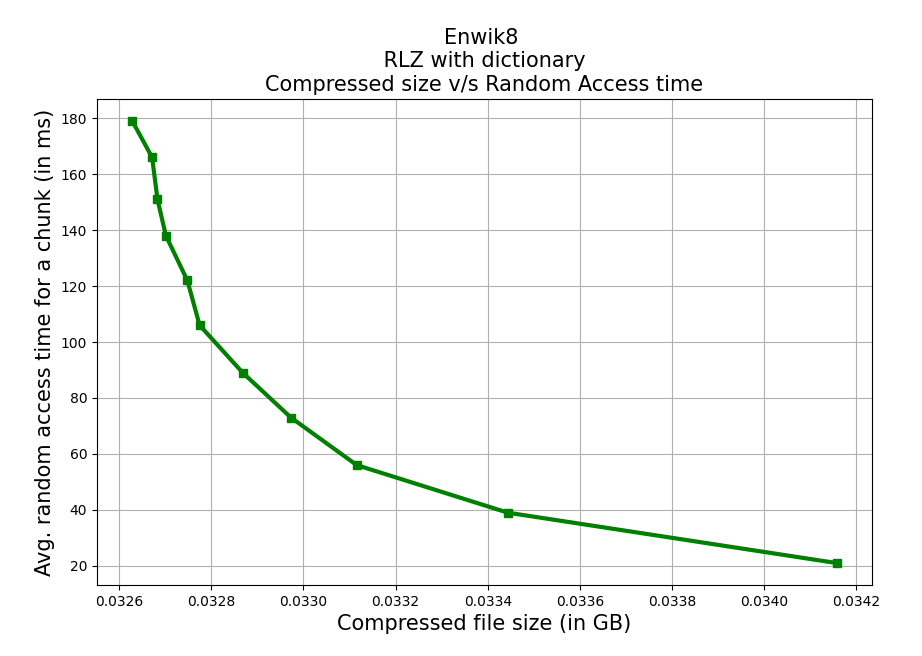
\includegraphics[width=\textwidth/2]{Figs/Enwik8_RLZ_dict.png}
    \caption{Compressed size v/s random access time for RLZ scheme with dictionary}
    \label{fig:enwik8_rlz_dict}
\end{figure}

\begin{figure}[H]
    \centering
    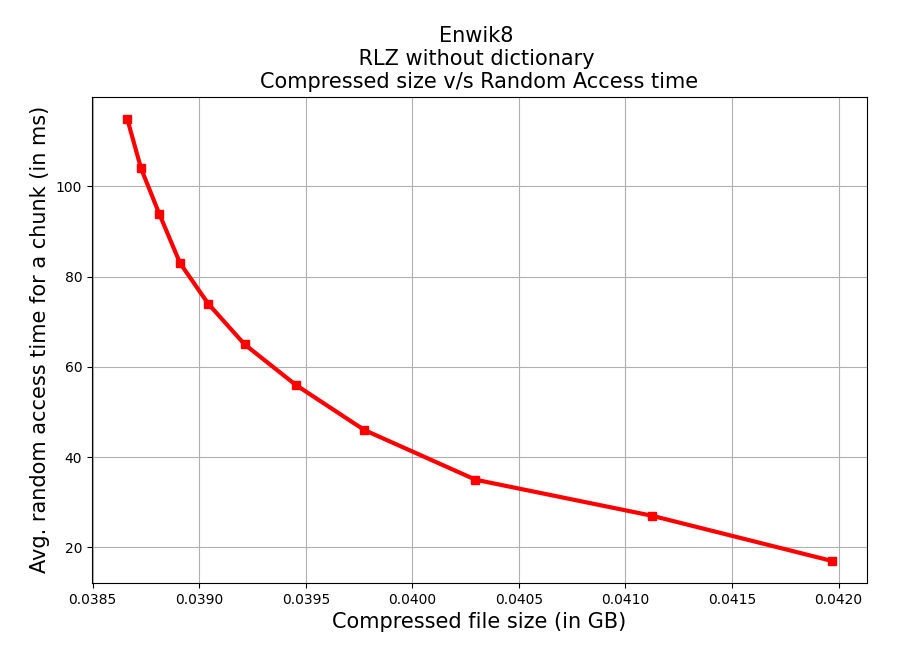
\includegraphics[width=\textwidth/2]{Figs/Enwik8_RLZ_nodict.png}
    \caption{Compressed size v/s random access time for RLZ scheme without dictionary}
    \label{fig:enwik8_rlz_nodict}
\end{figure}

From \href{fig:enwik8_rlz_dict}{fig-1} and \href{fig:enwik8_rlz_nodict}{fig-2} it can be observed that the RLZ scheme using a dictionary gives a smaller compressed file, but consumes more time for random access due to the additional overhead.

\begin{figure}[H]
    \centering
    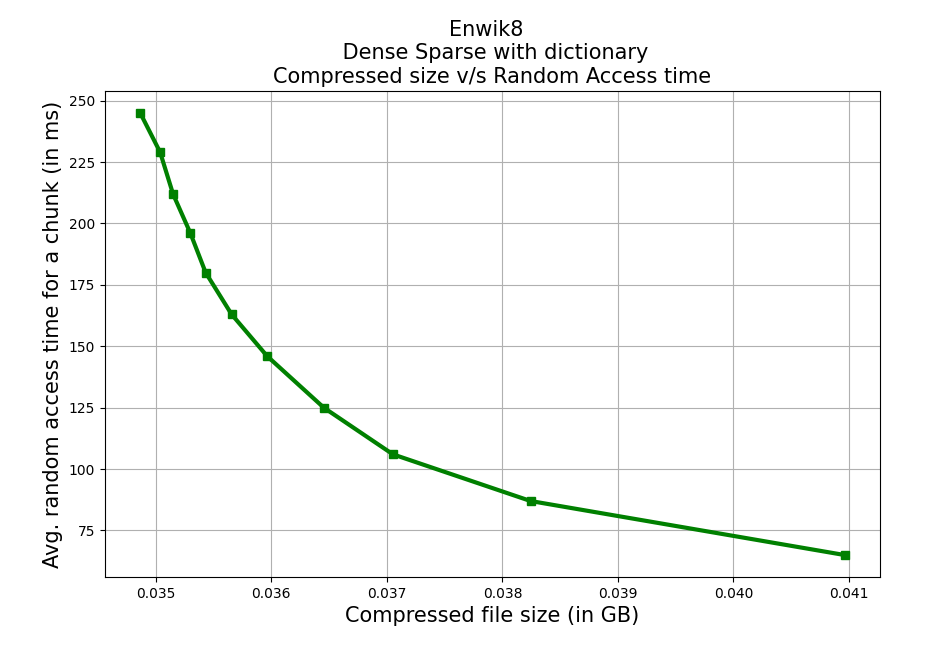
\includegraphics[width=\textwidth/2]{Figs/Enwik8_DS_dict.png}
    \caption{Compressed size v/s random access time for Dense-sparse scheme with dictionary}
    \label{fig:enwik8_ds_dict}
\end{figure}
\begin{figure}[H]
    \centering
    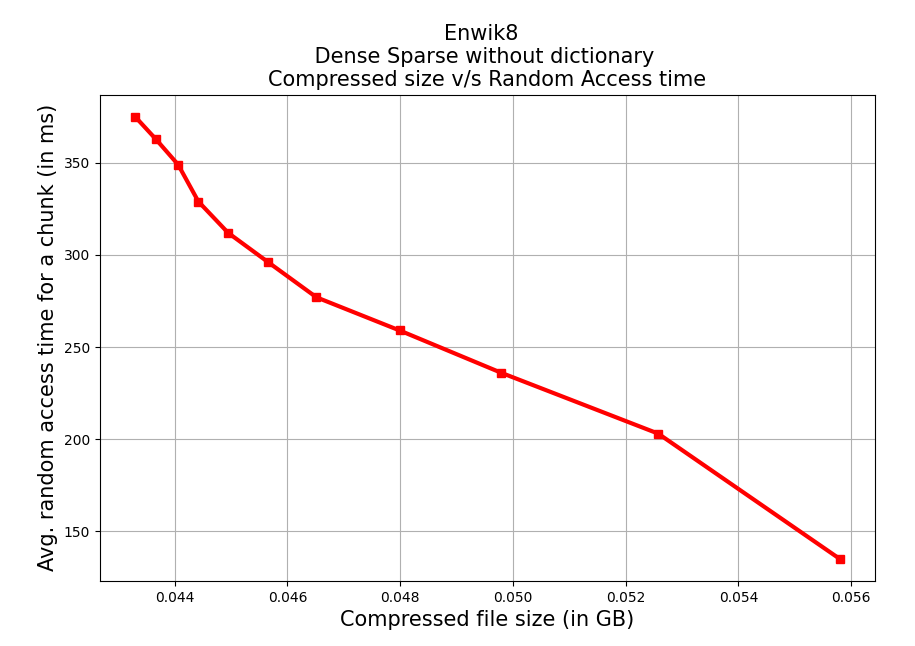
\includegraphics[width=\textwidth/2]{Figs/Enwik8_DS_nodict.png}
    \caption{Compressed size v/s random access time for Dense-sparse scheme without dictionary}
    \label{fig:enwik8_ds_nodict}
\end{figure}
From \href{fig:enwik8_ds_dict}{fig-3} and \href{fig:enwik8_ds_nodict}{fig-4} it can be observed that the dense-sparse scheme using a dictionary gives a smaller compressed file and consumes less time for random access, because of the smaller compressed size of each chunk and thereby less random access time.

\begin{figure}[H]
    \centering
    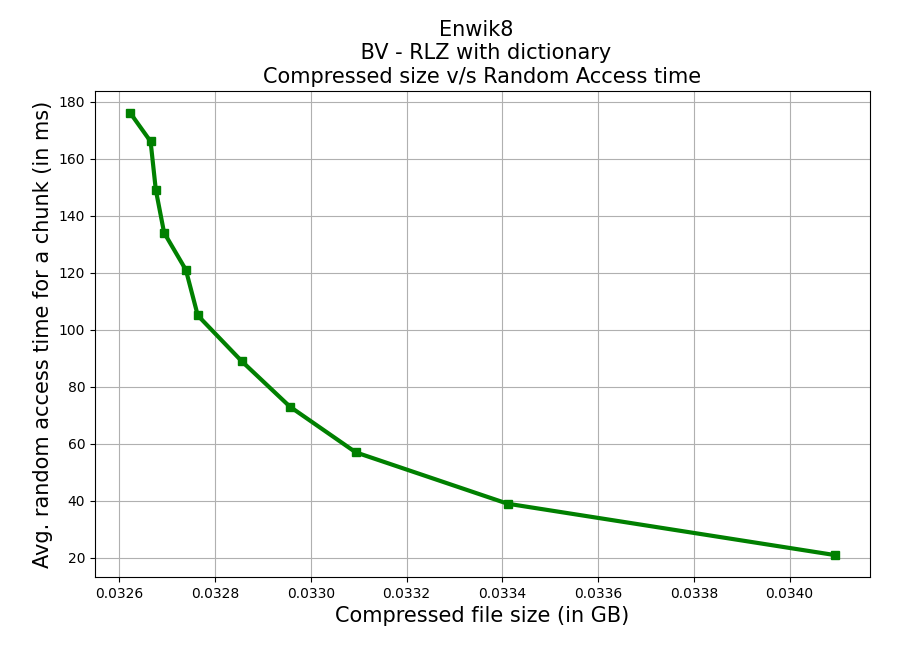
\includegraphics[width=\textwidth/2]{Figs/Enwik8_BV_RLZ_dict.png}
    \caption{Compressed size v/s random access time for BV-RLZ scheme with dictionary}
    \label{fig:enwik8_bv_rlz_dict}
\end{figure}


\begin{figure}[H]
    \centering
    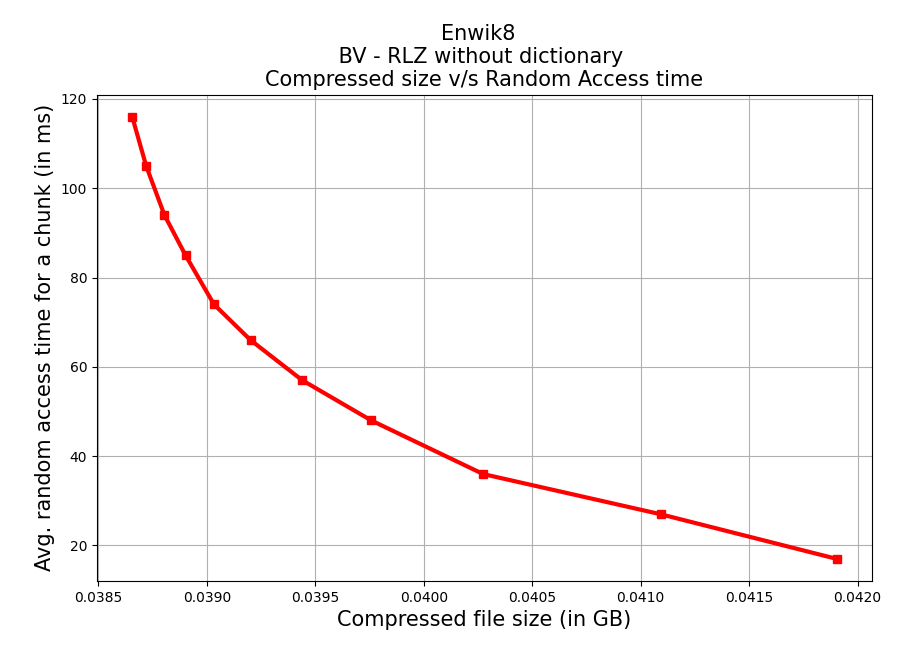
\includegraphics[width=\textwidth/2]{Figs/Enwik8_BV_RLZ_nodict.png}
    \caption{Compressed size v/s random access time for BV-RLZ scheme without dictionary}
    \label{fig:enwik8_bv_rlz_nodict}
\end{figure}

From \href{fig:enwik8_bv_rlz_dict}{fig-5} and \href{fig:enwik8_bv_rlz_nodict}{fig-6} a conclusion similar to the RLZ scheme can be derived.
\\~\\
Further, a custom method \verb|get(start, length)| was implement to optimize the random access time in dense-sparse scheme. The method returns the subsequence $Y[start \ldots start + length - 1]$ from $C_Y$, where $C_Y$ is the compressed bit-vector corresponding to the bit-vector $Y$. Suppose that we need to access a subsequence of length $k$ in the compressed bit-vector $C_Y$. Traditionally, using the random access operator \verb|[]| pre-defined in the SDSL library, the number of computations required is $\mathcal{O}(k (t_{select} + n / m))$ , where $m$ is the number of zeroes in the original bit vector $Y$. The custom method achieves this using $\mathcal{O}(t_{select} + kn / m)$ computations by using a single \verb|select()| method call.

\begin{figure}[H]
    \centering
    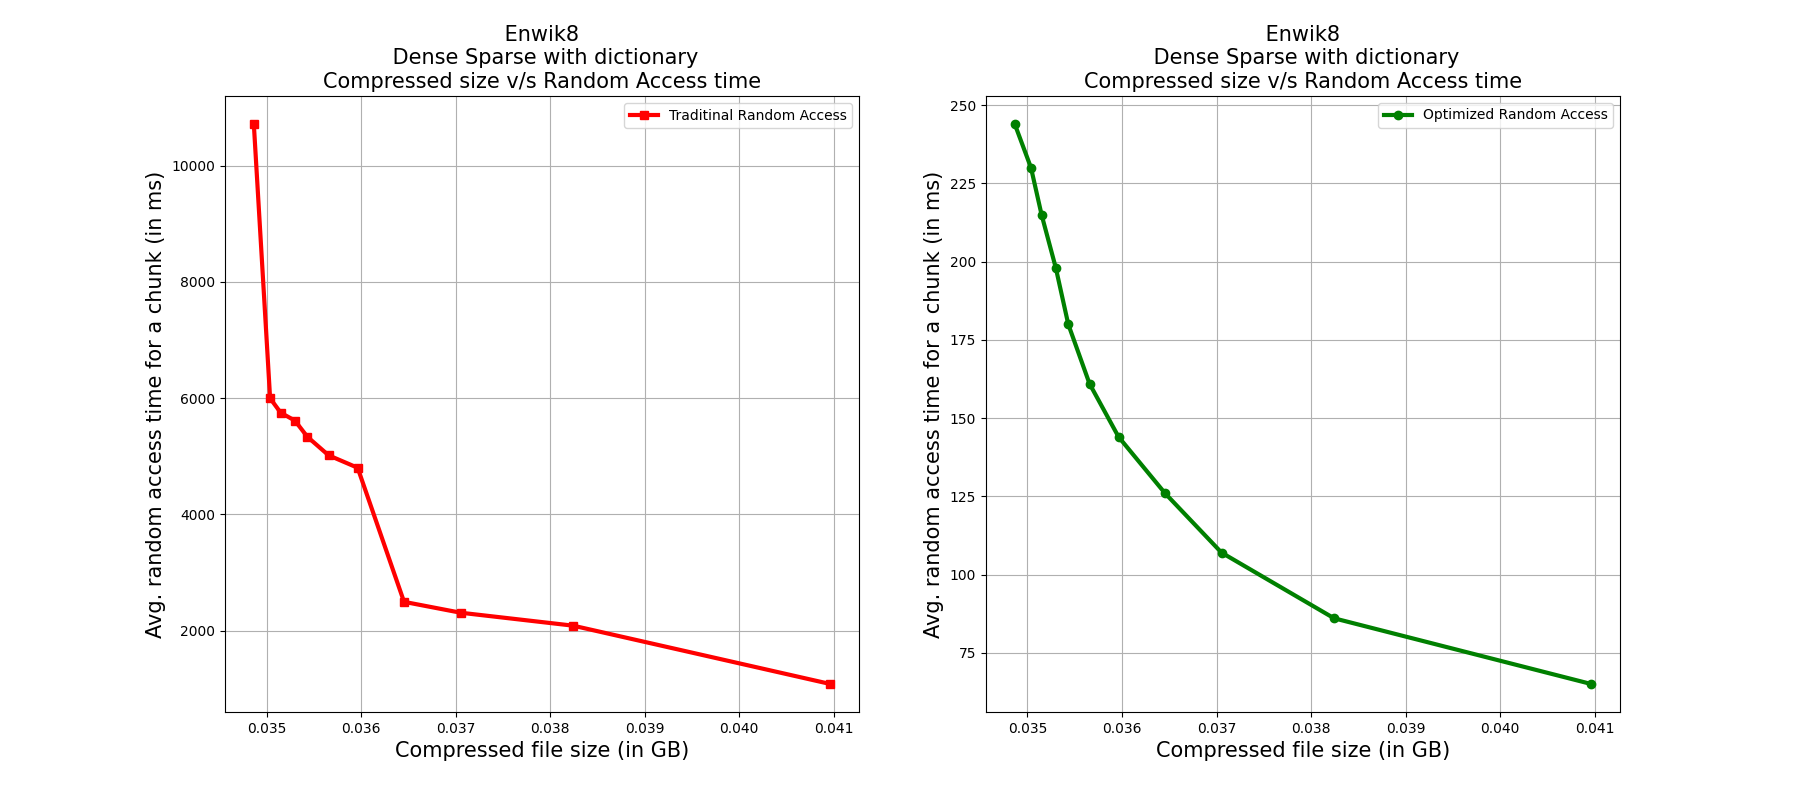
\includegraphics[width=\textwidth]{Figs/ds_opt.png}
    \caption{Compressed size v/s random access time for dense-sparse scheme using the traditional and optimized random access}
    \label{fig:ds_opt}
\end{figure}

From \href{fig:ds_opt}{fig-7}, a significant improvement in random access time can be observed using the optimized random access, while the compressed file size remains same. 

The source codes, instructions to run and text file links are in the following \href{https://github.com/srikanth2001/IDP_EE4015}{repository}